% 1993_新科目组_文科/figures/f1993_new_arts_q23_fold.tex — 1993 年·新科目组·文科 第 23 题（折叠正方形示意）
%
% 【来源】`.work/phase4-b17/source/1993新科目组文.pdf`（SHA-256 87609fbbfde93fee975f27833c96e2827b10934eb403dc01c4fcbb68c68e6a0a），第 1 页；
%   内容流 `q 1 0 0 1 529.958 70.754 cm` 段逐路径照录，
%   解析脚本 `.work/phase4-b17/probe/pdfparse_full.py`。
%
% 【坐标口径】源 PDF 用户空间（原点左下、y 向上）。本图本地坐标
%   (x,y) = (x_page − 529.958, y_page − 70.754)，1 单位 = 1 TeX pt。
%   线宽 0.398pt；虚线 [2.989 2.989] 0 d。
%
% 元素计数：实线 10 段（正方体四边、折叠后 D′C′/D′E′/C′E′/PE/PD′/PC′）+ 虚线 2 段（DE、CE）+ 9 个标签。
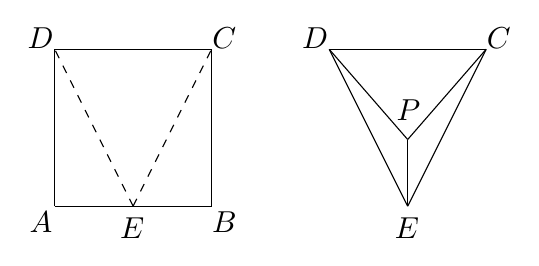
\begin{tikzpicture}[x=1pt, y=1pt,
    every node/.style={inner sep=0pt, font=\fontsize{10.5pt}{12.6pt}\selectfont}]
  \draw[line width=0.398pt] (0.000,0.000) -- (56.694,0.000);
  \draw[line width=0.398pt] (56.694,56.694) -- (56.694,0.000);
  \draw[line width=0.398pt] (56.694,56.694) -- (0.000,56.694);
  \draw[line width=0.398pt] (0.000,0.000) -- (0.000,56.694);
  \draw[line width=0.398pt] (99.214,56.694) -- (127.561,0.000);
  \draw[line width=0.398pt] (155.907,56.694) -- (127.561,0.000);
  \draw[line width=0.398pt] (155.907,56.694) -- (99.214,56.694);
  \draw[line width=0.398pt] (127.561,24.095) -- (127.561,0.000);
  \draw[line width=0.398pt] (127.561,24.095) -- (99.214,56.694);
  \draw[line width=0.398pt] (127.561,24.095) -- (155.907,56.694);
  % 虚线：正方形内 DE、CE（折痕）
  \draw[line width=0.398pt, dash pattern=on 2.989pt off 2.989pt] (28.347,0.000) -- (0.000,56.694);
  \draw[line width=0.398pt, dash pattern=on 2.989pt off 2.989pt] (28.347,0.000) -- (56.694,56.694);
  \node[anchor=center] at (-5.070,60.770) {$D$};
  \node[anchor=center] at (61.250,60.770) {$C$};
  \node[anchor=center] at (-4.930,-5.780) {$A$};
  \node[anchor=center] at (28.050,-7.820) {$E$};
  \node[anchor=center] at (61.360,-5.780) {$B$};
  \node[anchor=center] at (94.140,60.770) {$D$};
  \node[anchor=center] at (160.470,60.770) {$C$};
  \node[anchor=center] at (127.830,34.700) {$P$};  % 相对源中心上移 2.49pt、右移 1.0pt，避开 D–P 边
  \node[anchor=center] at (127.260,-7.820) {$E$};
\end{tikzpicture}
%
% 【自验结果】探针：坐标逐点照录内容流；与 400 dpi 渲染并排比对（标签位置取 pdftotext -bbox 中心）。
